\section{Descripción del lugar de estudio}\label{sec:lugar}

El establecimiento es el edificio de Servicios Complementarios de la Cooperativa Agrícola Industrial y de Servicios Múltiples El General (CoopeAgri R.L.), en San Isidro de El General, Pérez Zeledón. Su servicio eléctrico corresponde al NISE 2471778 del Instituto Costarricense de Electricidad (ICE) \cite{ice_facturas}. La Tabla~\ref{tab:sitio} resume la información general del sitio.

\begin{table}[!htb]
\caption{Información general del sitio}
\label{tab:sitio}
\centering
\footnotesize
\setlength{\tabcolsep}{3pt}
\begin{tabular}{l l}
\toprule
Parámetro & Valor \\
\midrule
Servicio & CoopeAgri R.L., Servicios Complementarios \\
NISE / medidor & 2471778 / 2092972 \\
Ubicación & San Isidro de El General, Pérez Zeledón \\
Coordenadas & \ang{9;22;37.0}\,N, \ang{83;42;6.8}\,O \\
Elevación & \SI{704}{m} s.\,n.\,m. \\
Tarifa & T-CO (comercio y servicios), no horaria \\
Acometida & Trifásica, 120/\SI{208}{V} \\
Techo disponible & \SI{1990}{m^2}, lámina metálica, $\approx\SI{0}{\degree}$ \\
Orientación del techo & Eje largo a $\approx\SI{7}{\degree}$ del norte--sur \\
Horario de atención & Lunes a sábado, 6:00 a 21:00 \\
\bottomrule
\end{tabular}
\end{table}

\subsection{Características de la zona}

San Isidro de El General está en el valle de El General, en la vertiente del Pacífico sur. La temperatura media mensual se mantiene entre \SI{21}{\celsius} y \SI{23}{\celsius}, y los extremos horarios entre 2005 y 2025 van de \SI{14.1}{\celsius} a \SI{30.5}{\celsius} \cite{nasa_power, nasa_power_horario}; estos valores se usan en la Sección~\ref{sec:modulo} para calcular las tensiones extremas de las cadenas. Hay una época seca de diciembre a abril y una lluviosa, con más nubosidad, de mayo a noviembre.

\subsection{Ubicación (vista satelital)}

La Fig.~\ref{fig:ubicacion} muestra la ubicación del edificio, en el sector norte del centro de San Isidro.

\begin{figure}[!htb]
\centering
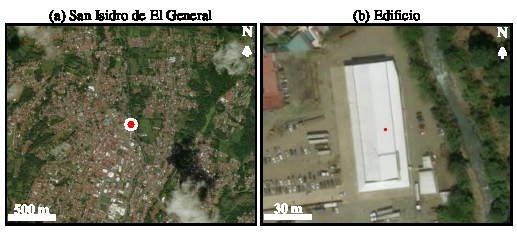
\includegraphics[width=\anchofig]{ubicacion_satelital.pdf}
\caption{Vista satelital del sitio de estudio ($9.37695^\circ$~N, $83.70189^\circ$~O): (a) ubicación en San Isidro de El General; (b) edificio de Servicios Complementarios (punto rojo).}
\label{fig:ubicacion}
\end{figure}

\subsection{Techo disponible}

Para el diseño se considera la parte central y más alta de la cubierta, de lámina metálica, con un área de \SI{1990}{m^2} y una inclinación cercana a \SI{0}{\degree}. A partir de la imagen satelital, esta superficie mide aproximadamente \SI{21.5}{m} de este a oeste y \SI{92.5}{m} de norte a sur. El eje largo del techo no está exactamente en la dirección norte--sur: en la imagen está girado unos \SI{7}{\degree}, con su extremo sur desplazado hacia el este. Por ser la parte más alta del edificio, no recibe sombra de los niveles más bajos de la cubierta.

\subsection{Caracterización del consumo eléctrico}

El servicio está en la tarifa T-CO, que cobra por separado la energía consumida y la demanda máxima del mes. La Tabla~\ref{tab:consumo} y la Fig.~\ref{fig:consumo} presentan los doce meses de setiembre de 2025 a agosto de 2026 \cite{ice_facturas}.

\begin{table}[!htb]
\caption{Consumo, demanda, factor de potencia y monto facturado (set.\ 2025 -- ago.\ 2026)}
\label{tab:consumo}
\centering
\footnotesize
\setlength{\tabcolsep}{3.5pt}
\begin{tabular}{l S[table-format=6.0] S[table-format=2.2] S[table-format=1.2] S[table-format=8.0]}
\toprule
{Mes} & {Energía [kWh]} & {Demanda [kW]} & {F.P.} & {Monto [¢]} \\
\midrule
Set. 2025 & 18238 & 53.00 & 0.95 & 2197090 \\
Oct. 2025 & 18727 & 47.12 & 0.98 & 2160335 \\
Nov. 2025 & 17993 & 44.92 & 0.98 & 2071120 \\
Dic. 2025 & 18972 & 44.31 & 0.98 & 2143700 \\
Ene. 2026 & 18482 & 43.70 & 0.96 & 1784895 \\
Feb. 2026 & 17626 & 49.33 & 0.98 & 1787605 \\
Mar. 2026 & 18238 & 45.78 & 0.98 & 1790965 \\
Abr. 2026 & 18850 & 46.14 & 0.98 & 1837895 \\
May. 2026 & 19339 & 46.88 & 0.98 & 1880430 \\
Jun. 2026 & 18482 & 45.78 & 0.98 & 1808075 \\
Jul. 2026 & 18972 & 44.19 & 0.98 & 1824720 \\
Ago. 2026 & 19094 & 47.25 & 0.98 & 1867375 \\
\midrule
Total     & 223013 & {--} & {--} & 23154205 \\
Promedio  & 18584  & 46.53 & {--} & 1929517 \\
\bottomrule
\end{tabular}
\end{table}

\begin{figure}[!htb]
\centering
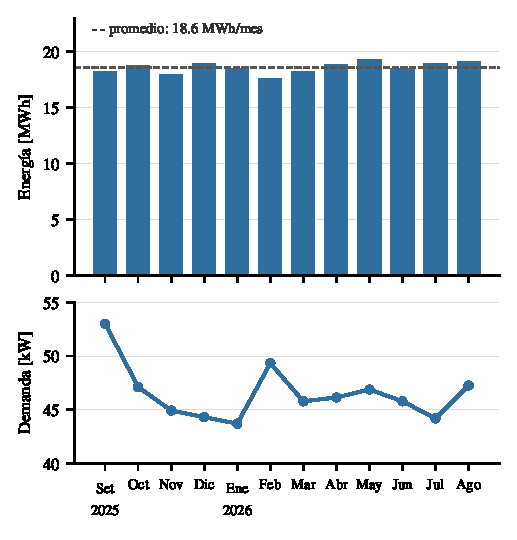
\includegraphics[width=\anchofig]{consumo_mensual.pdf}
\caption{Energía consumida (arriba) y demanda máxima (abajo) por mes de facturación.}
\label{fig:consumo}
\end{figure}

El consumo anual fue de \SI{223013}{kWh}, con un promedio de \SI{18584}{kWh} por mes. La variación entre meses es pequeña (desviación estándar del 2.7\,\%), así que las diferencias entre la generación y el consumo de cada mes dependerán casi solo de la radiación solar. Algunos valores de la Tabla~\ref{tab:consumo} se repiten porque todos los registros son múltiplos de la constante del medidor (\SI{122.4}{kWh}). La demanda máxima estuvo entre \SI{43.7}{kW} y \SI{53.0}{kW}.

En agosto de 2026 la energía representó el 61\,\% del monto facturado, la demanda el 25\,\%, el impuesto de valor agregado el 11\,\%, y el alumbrado público y el tributo de bomberos el 3\,\% restante \cite{ice_facturas}. Como el cargo por demanda depende de la demanda máxima del mes, el sistema no necesariamente lo reduce aunque disminuya la energía comprada; por eso, en el caso base de la evaluación económica se supone que no cambia.
